\documentclass{standalone}
\usepackage{tikz}
\usetikzlibrary{patterns, positioning}


\begin{document}
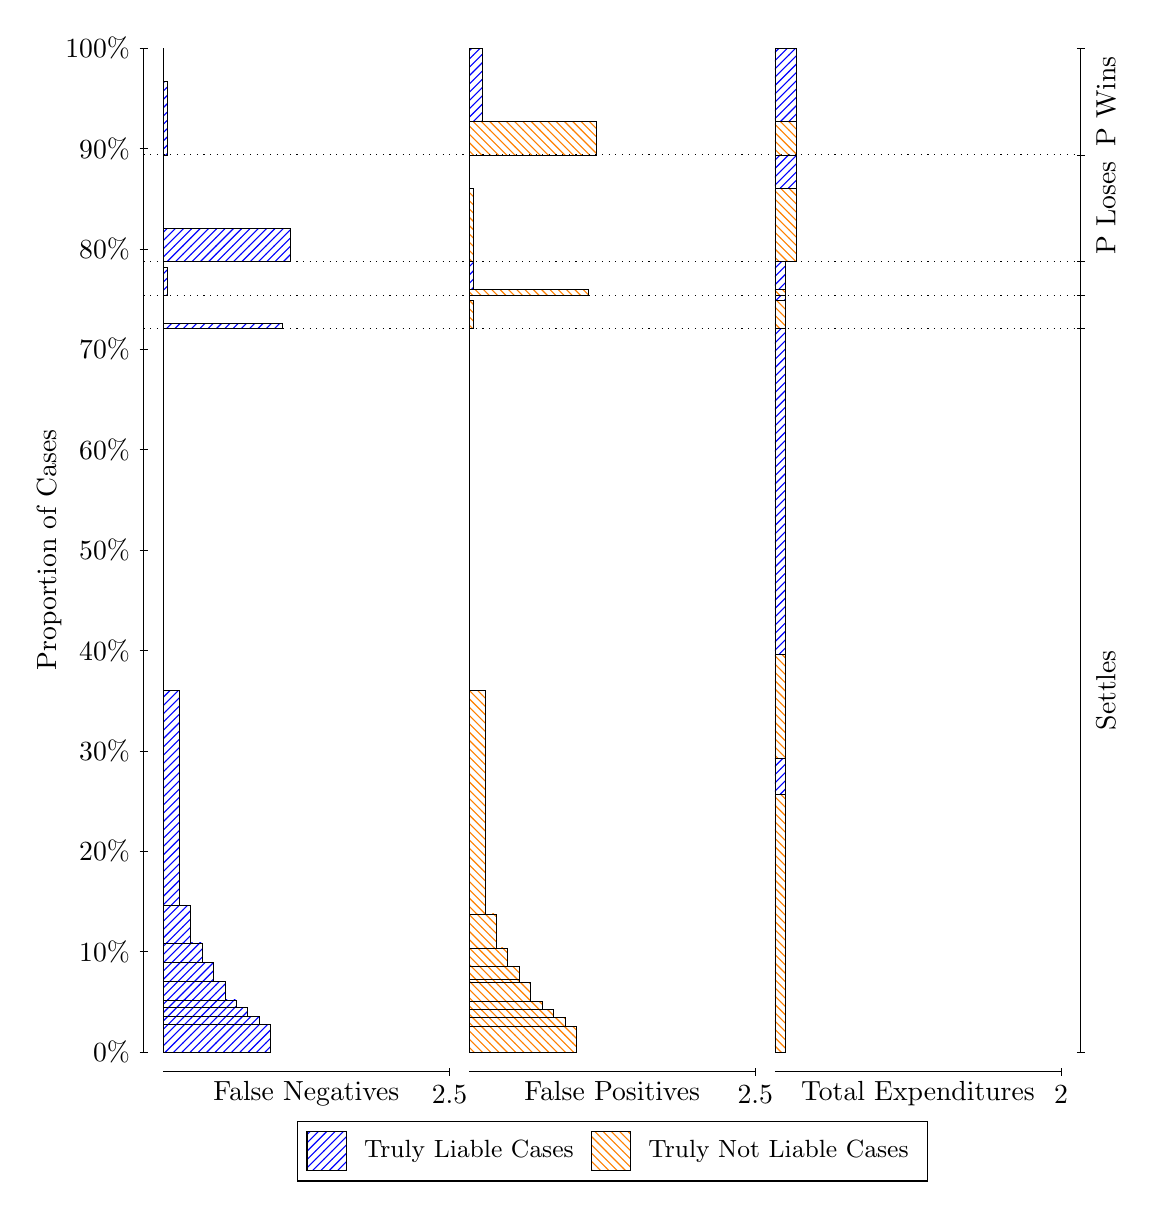
\begin{tikzpicture}
\draw[black, very thin] (1.5,1.75) -- (1.5,14.5);
\node[rotate=90, text=black, anchor=center] at (0.3, 8.125) {Proportion of Cases};
\draw[black, very thin] (1.45,1.75) -- (1.55,1.75);
\node[text=black, anchor=east] at (1.45, 1.75) {0\%};
\draw[black, very thin] (1.45,3.025) -- (1.55,3.025);
\node[text=black, anchor=east] at (1.45, 3.025) {10\%};
\draw[black, very thin] (1.45,4.3) -- (1.55,4.3);
\node[text=black, anchor=east] at (1.45, 4.3) {20\%};
\draw[black, very thin] (1.45,5.575) -- (1.55,5.575);
\node[text=black, anchor=east] at (1.45, 5.575) {30\%};
\draw[black, very thin] (1.45,6.85) -- (1.55,6.85);
\node[text=black, anchor=east] at (1.45, 6.85) {40\%};
\draw[black, very thin] (1.45,8.125) -- (1.55,8.125);
\node[text=black, anchor=east] at (1.45, 8.125) {50\%};
\draw[black, very thin] (1.45,9.4) -- (1.55,9.4);
\node[text=black, anchor=east] at (1.45, 9.4) {60\%};
\draw[black, very thin] (1.45,10.675) -- (1.55,10.675);
\node[text=black, anchor=east] at (1.45, 10.675) {70\%};
\draw[black, very thin] (1.45,11.95) -- (1.55,11.95);
\node[text=black, anchor=east] at (1.45, 11.95) {80\%};
\draw[black, very thin] (1.45,13.225) -- (1.55,13.225);
\node[text=black, anchor=east] at (1.45, 13.225) {90\%};
\draw[black, very thin] (1.45,14.5) -- (1.55,14.5);
\node[text=black, anchor=east] at (1.45, 14.5) {100\%};

\draw[black, very thin] (13.4,1.75) -- (13.4,14.5);
\draw[black, very thin] (13.35,1.75) -- (13.45,1.75);
\node[anchor=west] at (13.35, 1.75) {};
\draw[black, very thin] (13.35,10.937) -- (13.45,10.937);
\node[anchor=west] at (13.35, 10.937) {};
\draw[black, very thin] (13.35,11.362) -- (13.45,11.362);
\node[anchor=west] at (13.35, 11.362) {};
\draw[black, very thin] (13.35,11.787) -- (13.45,11.787);
\node[anchor=west] at (13.35, 11.787) {};
\draw[black, very thin] (13.35,13.143) -- (13.45,13.143);
\node[anchor=west] at (13.35, 13.143) {};
\draw[black, very thin] (13.35,14.5) -- (13.45,14.5);
\node[anchor=west] at (13.35, 14.5) {};

\draw[black, very thin, pattern color=blue, pattern=north east lines] (1.75,1.75) rectangle (3.1125,2.1047);
\draw[black, very thin, pattern color=blue, pattern=north east lines] (1.75,2.1047) rectangle (2.9672,2.2051);
\draw[black, very thin, pattern color=blue, pattern=north east lines] (1.75,2.2051) rectangle (2.8218,2.3135);
\draw[black, very thin, pattern color=blue, pattern=north east lines] (1.75,2.3135) rectangle (2.6765,2.4125);
\draw[black, very thin, pattern color=blue, pattern=north east lines] (1.75,2.4125) rectangle (2.5312,2.6509);
\draw[black, very thin, pattern color=blue, pattern=north east lines] (1.75,2.6509) rectangle (2.3858,2.8889);
\draw[black, very thin, pattern color=blue, pattern=north east lines] (1.75,2.8889) rectangle (2.2405,3.135);
\draw[black, very thin, pattern color=blue, pattern=north east lines] (1.75,3.135) rectangle (2.0952,3.6103);
\draw[black, very thin, pattern color=blue, pattern=north east lines] (1.75,3.6103) rectangle (1.9498,6.3418);
\draw[black, very thin, pattern color=orange, pattern=north west lines] (1.75,6.3418) rectangle (1.75,10.937);
\draw[black, very thin, pattern color=blue, pattern=north east lines] (1.75,10.937) rectangle (3.2578,11.007);
\draw[black, very thin, pattern color=orange, pattern=north west lines] (1.75,11.007) rectangle (1.75,11.362);
\draw[black, very thin, pattern color=blue, pattern=north east lines] (1.75,11.362) rectangle (1.8045,11.718);
\draw[black, very thin, pattern color=orange, pattern=north west lines] (1.75,11.718) rectangle (1.75,11.787);
\draw[black, very thin, pattern color=blue, pattern=north east lines] (1.75,11.787) rectangle (3.3668,12.209);
\draw[black, very thin, pattern color=orange, pattern=north west lines] (1.75,12.209) rectangle (1.75,13.143);
\draw[black, very thin, pattern color=blue, pattern=north east lines] (1.75,13.143) rectangle (1.8045,14.078);
\draw[black, very thin, pattern color=orange, pattern=north west lines] (1.75,14.078) rectangle (1.75,14.5);
\draw[black, very thin, pattern color=orange, pattern=north west lines] (5.6333,1.75) rectangle (6.9958,2.0794);
\draw[black, very thin, pattern color=orange, pattern=north west lines] (5.6333,2.0794) rectangle (6.8505,2.1845);
\draw[black, very thin, pattern color=orange, pattern=north west lines] (5.6333,2.1845) rectangle (6.7052,2.2889);
\draw[black, very thin, pattern color=orange, pattern=north west lines] (5.6333,2.2889) rectangle (6.5598,2.3963);
\draw[black, very thin, pattern color=orange, pattern=north west lines] (5.6333,2.3963) rectangle (6.4145,2.6325);
\draw[black, very thin, pattern color=orange, pattern=north west lines] (5.6333,2.6325) rectangle (6.2692,2.6712);
\draw[black, very thin, pattern color=orange, pattern=north west lines] (5.6333,2.6712) rectangle (6.2692,2.8351);
\draw[black, very thin, pattern color=orange, pattern=north west lines] (5.6333,2.8351) rectangle (6.1238,3.0732);
\draw[black, very thin, pattern color=orange, pattern=north west lines] (5.6333,3.0732) rectangle (5.9785,3.5049);
\draw[black, very thin, pattern color=orange, pattern=north west lines] (5.6333,3.5049) rectangle (5.8332,6.3452);
\draw[black, very thin, pattern color=blue, pattern=north east lines] (5.6333,6.3452) rectangle (5.6333,10.937);
\draw[black, very thin, pattern color=orange, pattern=north west lines] (5.6333,10.937) rectangle (5.6878,11.292);
\draw[black, very thin, pattern color=blue, pattern=north east lines] (5.6333,11.292) rectangle (5.6333,11.362);
\draw[black, very thin, pattern color=orange, pattern=north west lines] (5.6333,11.362) rectangle (7.1412,11.43);
\draw[black, very thin, pattern color=blue, pattern=north east lines] (5.6333,11.43) rectangle (5.6878,11.787);
\draw[black, very thin, pattern color=orange, pattern=north west lines] (5.6333,11.787) rectangle (5.6878,12.721);
\draw[black, very thin, pattern color=blue, pattern=north east lines] (5.6333,12.721) rectangle (5.6333,13.143);
\draw[black, very thin, pattern color=orange, pattern=north west lines] (5.6333,13.143) rectangle (7.2502,13.565);
\draw[black, very thin, pattern color=blue, pattern=north east lines] (5.6333,13.565) rectangle (5.7968,14.5);
\draw[black, very thin, pattern color=orange, pattern=north west lines] (9.5167,1.75) rectangle (9.6529,5.022);
\draw[black, very thin, pattern color=blue, pattern=north east lines] (9.5167,5.022) rectangle (9.6529,5.4771);
\draw[black, very thin, pattern color=orange, pattern=north west lines] (9.5167,5.4771) rectangle (9.6529,6.8003);
\draw[black, very thin, pattern color=blue, pattern=north east lines] (9.5167,6.8003) rectangle (9.6529,10.937);
\draw[black, very thin, pattern color=orange, pattern=north west lines] (9.5167,10.937) rectangle (9.6529,11.292);
\draw[black, very thin, pattern color=blue, pattern=north east lines] (9.5167,11.292) rectangle (9.6529,11.362);
\draw[black, very thin, pattern color=orange, pattern=north west lines] (9.5167,11.362) rectangle (9.6529,11.43);
\draw[black, very thin, pattern color=blue, pattern=north east lines] (9.5167,11.43) rectangle (9.6529,11.787);
\draw[black, very thin, pattern color=orange, pattern=north west lines] (9.5167,11.787) rectangle (9.7892,12.721);
\draw[black, very thin, pattern color=blue, pattern=north east lines] (9.5167,12.721) rectangle (9.7892,13.143);
\draw[black, very thin, pattern color=orange, pattern=north west lines] (9.5167,13.143) rectangle (9.7892,13.565);
\draw[black, very thin, pattern color=blue, pattern=north east lines] (9.5167,13.565) rectangle (9.7892,14.5);
\draw[black, dotted] (1.5,10.937) -- (13.4,10.937);
\draw[black, dotted] (1.5,11.362) -- (13.4,11.362);
\draw[black, dotted] (1.5,11.787) -- (13.4,11.787);
\draw[black, dotted] (1.5,13.143) -- (13.4,13.143);
\draw[black, very thin] (1.75,1.5) -- (5.3833,1.5);
\node[text=black, anchor=north] at (3.5667, 1.5) {False Negatives};
\draw[black, very thin] (5.3833,1.45) -- (5.3833,1.55);
\node[text=black, anchor=north] at (5.3833, 1.45) {2.5};

\draw[black, very thin] (5.6333,1.5) -- (9.2667,1.5);
\node[text=black, anchor=north] at (7.45, 1.5) {False Positives};
\draw[black, very thin] (9.2667,1.45) -- (9.2667,1.55);
\node[text=black, anchor=north] at (9.2667, 1.45) {2.5};

\draw[black, very thin] (9.5167,1.5) -- (13.15,1.5);
\node[text=black, anchor=north] at (11.333, 1.5) {Total Expenditures};
\draw[black, very thin] (13.15,1.45) -- (13.15,1.55);
\node[text=black, anchor=north] at (13.15, 1.45) {2};

\node[text=black, centered, rotate=90] at (13.72, 6.3435) {Settles};


\node[text=black, centered, rotate=90] at (13.72, 12.465) {P Loses};
\node[text=black, centered, rotate=90] at (13.72, 13.822) {P Wins};

\draw (7.449999999999999,1.5) node[draw=none] (baseCoordinate) {};
\begin{scope}[align=center]
        \matrix[scale=0.5, draw=black, below=0.5cm of baseCoordinate, nodes={draw}, column sep=0.1cm]{
            \node[rectangle, draw, minimum width=0.5cm, minimum height=0.5cm, pattern color=blue, pattern=north east lines] {}; &
            \node[draw=none, font=\small, text=black] (B) {Truly Liable Cases}; &
            \node[rectangle, draw, minimum width=0.5cm, minimum height=0.5cm, pattern color=orange, pattern=north west lines] {}; &
            \node[draw=none, font=\small, text=black] (B) {Truly Not Liable Cases}; \\
            };
\end{scope}

\end{tikzpicture}
\end{document}